\documentclass[11pt]{amsart}
\usepackage[margin=1.1in]{geometry}
\usepackage{amsmath,amssymb,amsthm,mathtools,booktabs,tikz}
\usepackage[hidelinks]{hyperref}

\newtheorem{theorem}{Theorem}
\newtheorem{lemma}[theorem]{Lemma}
\newtheorem{proposition}[theorem]{Proposition}
\newtheorem{corollary}[theorem]{Corollary}
\theoremstyle{remark}
\newtheorem{remark}[theorem]{Remark}

\newcommand{\Vd}{V_\delta}
\DeclareMathOperator{\dist}{dist}

\title[Shrinking tubes around a circular billiard orbit]{Shrinking tubes around a circular billiard orbit:\\ spatial dephasing and arithmetic oscillation of the uncovered area}
\author{[Author name and affiliation to be supplied by the author]}
\date{Draft of 14 November 2026}

\begin{document}

\begin{abstract}
Fix an irrational rotation angle and follow the first $N$ chords of a circular
billiard orbit in the unit disk. We study the normalized area $V_N(c)$ of the part of
the disk at distance more than $c/N$ from these chords. We prove that, as
$N\to\infty$, $V_N(c)$ is asymptotically equal to the area $a^2$ of the caustic disk
plus a radial integral of the \emph{square} of the uncovered length of the circle by
$N$ arcs of half-length proportional to $1/N$ centred at the rotation orbit. The
square arises only after radial integration; the two angular branches through a
point are not independent. Combined with the three-distance theorem this gives: (i)
for every irrational angle, $\liminf V_N(c)$ is at least an explicit uniform-gap value
$\Vd(c)$, with equality exactly when the angle has unbounded partial quotients, in
which case $V_N(c)$ diverges for every $c>0$; (ii) for the golden angle (and every
noble angle) the full set of limit points of $V_N(c)$ is an explicit interval, its
lower end is attained along Fibonacci times by a convex-order argument, and
$V_N(c)$ converges if and only if $c\ge c_*=\pi\sin\alpha/(\sqrt5\lambda^3)$.
Finite-$N$ Monte Carlo and deterministic computations agree with the limits.
\end{abstract}

\maketitle

\section{Introduction}

Let $D$ be the closed unit disk, $0<\alpha<\pi/2$, and $\beta=\alpha/\pi\notin\mathbb Q$.
The billiard orbit starting at $p_0=(1,0)$ with reflection angle determined by $\alpha$
visits $p_j=(\cos 2j\alpha,\sin 2j\alpha)$. Let
\[
\Gamma_N=\bigcup_{j=0}^{N-1}[p_j,p_{j+1}]
\]
be the union of its first $N$ complete chords. Every chord is tangent to the caustic
circle of radius $a=\cos\alpha$, the chord normals are $u_j=(\cos\theta_j,\sin\theta_j)$
with $\theta_j=(2j+1)\alpha$, and chord $j$ lies on the line $u_j\cdot x=a$. Put
$Q=\sin\alpha$. For $c>0$ define the vacancy
\[
V_N(c)=\frac{1}{\pi}\,\bigl|\{x\in D:\dist(x,\Gamma_N)>c/N\}\bigr|,
\]
where $\dist$ is distance to the finite segments and $c/N$ is a tube \emph{half}-width.
The caustic disk is never entered, so $V_N(c)\ge (a-c/N)^2$. The total length of
$\Gamma_N$ grows like $N$, so a width of order $1/N$ is the scale at which the covered
fraction of the outer annulus $a<|x|<1$ is nontrivial.

The rotation orbit $\{\theta_j\}_{j<N}$ has circular gaps $g_{N,0},\dots,g_{N,N-1}$
summing to $2\pi$. The uncovered fraction of the circle by the closed arcs of
half-length $s/N$ centred at these points is
\begin{equation}\label{eq:mN}
m_N(s)=\frac{1}{2\pi}\sum_{j=0}^{N-1}\Bigl(g_{N,j}-\frac{2s}{N}\Bigr)_+ .
\end{equation}

\begin{theorem}[Spatial dephasing]\label{thm:A}
For fixed irrational $\beta\in(0,1/2)$ and fixed $c>0$,
\[
V_N(c)=a^2+2\int_0^{Q} q\,m_N(c/q)^2\,dq+o(1)\qquad(N\to\infty).
\]
\end{theorem}

Equivalently, with $q=\sqrt{r^2-a^2}$, $V_N(c)=a^2+2\int_a^1 r\,m_N\bigl(c/\sqrt{r^2-a^2}\bigr)^2dr+o(1)$.
A point at radius $r>a$ is covered if and only if one of two angular branches,
$\varphi\pm\arccos(a/r)$, is close to the rotation orbit. The two branches are coupled
deterministically; at a fixed radius their joint vacancy is an autocorrelation of the
circle vacancy indicator, not a product. Radial averaging over the lag $2\arccos(a/r)$
removes every nonzero Fourier mode, which is why only the square of the mean survives.
No rate is claimed.

Write $\Vd(c)=a^2+2\int_0^Q q\,(1-c/(\pi q))_+^2\,dq$, the value the right-hand side of
Theorem~\ref{thm:A} would take if all gaps were equal. Explicitly,
$\Vd(c)=a^2+Q^2-4cQ/\pi+3(c/\pi)^2+2(c/\pi)^2\log(\pi Q/c)$ for $0<c<\pi Q$ and
$\Vd(c)=a^2$ for $c\ge\pi Q$.

\begin{theorem}[Uniform-gap envelope]\label{thm:C}
Let $\beta\in(0,1/2)$ be irrational with partial quotients $(a_k)$ and let $c>0$.
\begin{enumerate}
\item $\liminf_N V_N(c)\ge \Vd(c)$.
\item If $(a_k)$ is unbounded, then $\liminf_N V_N(c)=\Vd(c)$ and $\limsup_N V_N(c)\ge W(c)>\Vd(c)$, where
$W(c)=a^2+2\int_0^Q q\,[(\tfrac12-\tfrac{c}{\pi q})_++\tfrac12]^2dq$. In particular $V_N(c)$ diverges for every $c>0$.
\item If $(a_k)$ is bounded and $0<c<\pi Q$, then $\liminf_N V_N(c)>\Vd(c)$.
\end{enumerate}
\end{theorem}

\begin{corollary}
For any fixed $c\in(0,\pi\sin\alpha)$, the angle $\beta$ is badly approximable if and
only if $\liminf_N V_N(c)>\Vd(c)$.
\end{corollary}

For the golden angle the limit set can be computed exactly. Let $\lambda=(\sqrt5-1)/2$,
$\beta=\lambda^2$, $u=\pi/(\sqrt5\lambda^2)$, and for $x\in[0,\lambda]$ let $\mu_x$ be the
law with atoms $\ell_i=u(1+x)\lambda^i$ and weights
$f=(\lambda-x,\lambda^2+x,x)/(1+x)$, $i=0,1,2$. Put
\[
M_x(s)=\frac1\pi\sum_{i=0}^{2}f_i(\ell_i-s)_+,\qquad
V(x,c)=a^2+2\int_0^Q q\,M_x(c/q)^2\,dq .
\]

\begin{theorem}[Golden angle]\label{thm:B}
Let $\beta=\lambda^2$ and $c>0$. Then
\begin{enumerate}
\item the set of limit points of $V_N(c)$ is the interval $\{V(x,c):x\in[0,\lambda]\}$;
\item $\liminf_N V_N(c)=V(0,c)=\lim_{m\to\infty}V_{F_m}(c)$, where $F_m$ are the Fibonacci numbers;
\item $V(x,c)>V(0,c)$ if and only if $0<x<\lambda$ and $c<Qu(1+x)$. Consequently
$\limsup_N V_N(c)>\liminf_N V_N(c)$ if and only if $c<c_*=Qu/\lambda=\pi Q/(\sqrt5\lambda^3)\approx 5.547$, and $V_N(c)\to a^2$ for $c\ge c_*$.
\end{enumerate}
The same conclusions hold, with $a=\cos\pi\beta$ and $Q=\sin\pi\beta$, for every
noble $\beta\in(0,1/2)$, i.e.\ every $\beta$ whose partial quotients are eventually $1$.
\end{theorem}

For $Qu\le c<c_*$ (about $3.428\le c<5.547$) the outer annulus is asymptotically fully
covered along Fibonacci times, while along other times a positive area stays
uncovered. Certified values (interval arithmetic, Section~\ref{sec:golden}) are
$V(0,1)=0.3362261295\ldots$, $V(1/3,1)=0.3381403717\ldots$, $V(0,2)=0.1564616538\ldots$,
$V(1/3,2)=0.1621730101\ldots$.

\paragraph{Relation to prior work.}
The caustic of the circular billiard and the three-distance theorem
\cite{Sos58,Swier59,Slater67,vRav88,AB98,Leong17} are classical, and the fixed-angle
gap and hitting-time laws of irrational rotations, including their failure to converge
along the full sequence, are well studied \cite{CdF96,Coelho04,BI09,DK24}. Hitting-time
statistics for integrable billiards \cite{DMS17} assume an absolutely continuous family
of frequencies and do not apply to a single fixed angle; cover times of rotations
\cite{Zhao25} are a different observable. Fixed-direction free path lengths in the
periodic Lorentz gas lead to area computations driven by three-strip structure
\cite{MS03,BZ07}, which is closest in spirit. We did not find the planar tube-vacancy
statements above in the literature we could access; this is a bounded search, and the
underlying ingredients (almost invariance, Riemann--Lebesgue, three-distance arithmetic,
convex order) are standard. For Theorem~\ref{thm:C}, the closest one-dimensional statements are Coelho and de Faria's
dichotomy between uniform and piecewise linear subsequential entrance-time laws
\cite[Thm.~I]{CdF96}, Coelho's result that tightness of rescaled hitting-time processes holds
exactly for bounded type \cite{Coelho04}, and the classical fact that gap ratios of $\{n\beta\}$
stay bounded exactly for badly approximable $\beta$ (see e.g.\ \cite[\S4]{Ram14}).
Theorem~\ref{thm:C} transfers such a dichotomy to the planar area observable; we did not find
this planar form, nor the golden phase family with its convex-order minimality, in
\cite{CdF96} (full text read) or elsewhere, but we could not read \cite{Coelho04,DK24} in full.
Our contribution is the exact reduction of the planar
observable to the one-dimensional gap law and the resulting arithmetic consequences.

\section{Exact two-branch structure}\label{sec:geometry}

Fix $\varepsilon\in(0,(1-a)/3)$, write $I_\varepsilon=[a+\varepsilon,1-\varepsilon]$ and
$w=c/N$, and take $N$ large enough that $w<\min(\varepsilon/2,a)$ and $(1-\varepsilon)^2-(a-w)^2<Q^2$.

\begin{lemma}\label{lem:branches}
For $r\in I_\varepsilon$ let $d_\mp(r)=\arccos((a\pm w)/r)$. A point $x=re^{i\varphi}$ satisfies
$\dist(x,\Gamma_N)\le w$ if and only if $\varphi-\theta_j\in\pm[d_-(r),d_+(r)]\pmod{2\pi}$
for some $j<N$.
\end{lemma}

\begin{proof}
With $\delta=\varphi-\theta_j$, the distance to the line $u_j\cdot x=a$ is $|r\cos\delta-a|$,
so it is at most $w$ exactly when $|\delta|\in[d_-,d_+]$; here $(a+w)/r<1$. On that set
the coordinate of $x$ along the chord direction is $r|\sin\delta|\le\sqrt{r^2-(a-w)^2}<Q$,
while the chord occupies coordinates $[-Q,Q]$; hence the foot of the perpendicular lies
on the chord and the distance to the chord equals the distance to the line. Off that set
the distance to the chord is at least the distance to the line, which exceeds $w$.
\end{proof}

Let $F_{N,s}$ be the indicator of the points of the circle at circular distance more than
$s/N$ from every $\theta_j$, $j<N$, so that $\int F_{N,s}\,d\varphi/2\pi=m_N(s)$. With
$\bar d_N=(d_++d_-)/2$, $h_N=(d_+-d_-)/2$, $s_N=Nh_N$ and $\psi_N=2\bar d_N$,
Lemma~\ref{lem:branches} gives for the uncovered angular fraction at radius $r\in I_\varepsilon$
\begin{equation}\label{eq:autocorr}
U_N(r)=\int F_{N,s_N(r)}(\varphi-\bar d_N)\,F_{N,s_N(r)}(\varphi+\bar d_N)\,\frac{d\varphi}{2\pi}
=C_{N,s_N(r)}(\psi_N(r)),
\end{equation}
where $C_{N,s}(t)=\int F_{N,s}(\varphi)F_{N,s}(\varphi+t)\,d\varphi/2\pi$. Since
$(r,w)\mapsto\arccos((a\pm w)/r)$ is real analytic near $I_\varepsilon\times\{0\}$,
$s_N(r)\to c/q(r)$ uniformly with $q(r)=\sqrt{r^2-a^2}$, and $\psi_N\to\psi=2\arccos(a/r)$ in
$C^2(I_\varepsilon)$, where $\psi'=2a/(rq)\ge 2a/(1-\varepsilon)>0$.

\section{Proof of Theorem~\ref{thm:A}}

\emph{Layers.} If $r<a-w$ every line is at distance at least $a-r>w$, so $U_N(r)=1$.
The radii $[a-w,a+\varepsilon]\cup[1-\varepsilon,1]$ carry normalized area at most
$2(a+\varepsilon)(\varepsilon+w)+2\varepsilon$, both for $V_N$ and for the right-hand side
(since $0\le m_N\le1$). Hence
\[
\Bigl|V_N(c)-a^2-2\!\int_a^1\! r\,m_N(c/q)^2dr\Bigr|
\le 6\varepsilon+2w+\Bigl|\int_{I_\varepsilon}2r\bigl[C_{N,s_N(r)}(\psi_N(r))-m_N(c/q(r))^2\bigr]dr\Bigr|.
\]

\emph{Low modes.} Rotation by $2\alpha$ maps $\{\theta_0,\dots,\theta_{N-1}\}$ to
$\{\theta_1,\dots,\theta_N\}$, so $F_{N,s}(\cdot-2\alpha)$ and $F_{N,s}$ differ on at most
two arcs: $\|F_{N,s}(\cdot-2\alpha)-F_{N,s}\|_{L^1(d\varphi/2\pi)}\le 2s/(\pi N)$. For the
Fourier coefficients $\hat F_{N,s}(k)$ this gives
$|e^{-2ik\alpha}-1|\,|\hat F_{N,s}(k)|\le 2s/(\pi N)$. As $\beta\notin\mathbb Q$, for every
fixed $k\ne0$ we get $\sup_{s\le S}|\hat F_{N,s}(k)|\to0$.

\emph{High modes.} By Parseval, $\sum_k|\hat F_{N,s}(k)|^2=m_N(s)\le1$ and
$C_{N,s}(t)=\sum_k|\hat F_{N,s}(k)|^2e^{ikt}$ converges absolutely. For an interval
$J\subset I_\varepsilon$ and $k\ne0$, integration by parts and the uniform bounds on
$\psi_N'$ and $(2r/\psi_N')'$ give $|\int_J 2r\,e^{ik\psi_N(r)}dr|\le B_\varepsilon/|k|$,
uniformly in $J$ and large $N$. Hence for fixed $s\le S$,
\[
\Bigl|\int_J 2r\bigl[C_{N,s}(\psi_N(r))-m_N(s)^2\bigr]dr\Bigr|\le
2\!\sum_{0<|k|\le K}\!|\hat F_{N,s}(k)|^2+\frac{B_\varepsilon}{K},
\]
which tends to $0$ when $N\to\infty$ and then $K\to\infty$.

\emph{Unfreezing.} Moving $N$ arcs' half-widths from $s/N$ to $t/N$ changes $F$ on a set of
measure at most $|s-t|/\pi$, so $|C_{N,s}-C_{N,t}|\le2|s-t|/\pi$ and
$|m_N(s)^2-m_N(t)^2|\le2|s-t|/\pi$, uniformly in $N$ and the lag. Partition $I_\varepsilon$
into finitely many intervals on which $c/q$ oscillates by less than $\eta$, freeze $s$ on
each, and use $s_N\to c/q$ uniformly. The integral above is then at most
$8\eta/\pi+o(1)$. Letting $N\to\infty$, then $\eta\to0$, then $\varepsilon\to0$ proves the
theorem. \qed

\begin{remark}
The order of limits is: fix $\varepsilon$, then the partition, then the Fourier cutoff $K$,
let $N\to\infty$, then $K\to\infty$, refine the partition, and finally let
$\varepsilon\to0$. The rate in the low-mode step depends on the Diophantine properties of
$\beta$, which is why no rate is stated.
\end{remark}

\section{Gap laws and Theorem~\ref{thm:C}}

Write $\tilde V_N(c)=a^2+2\int_0^Qq\,m_N(c/q)^2dq$; by Theorem~\ref{thm:A},
$V_N(c)-\tilde V_N(c)\to0$. The quantities below depend only on the multiset of gaps.

\begin{lemma}[Jensen]\label{lem:jensen}
For all $N$ and $s\ge0$, $m_N(s)\ge(1-s/\pi)_+$; hence $\tilde V_N(c)\ge\Vd(c)$. For
$s\le\pi$, $2\pi\bigl(m_N(s)-(1-s/\pi)\bigr)=\sum_j(2s/N-g_{N,j})_+$.
\end{lemma}

\begin{proof}
$\sum_j(g_{N,j}-2s/N)_+\ge\max(0,\sum_j(g_{N,j}-2s/N))=(2\pi-2s)_+$. The identity follows from
$y_+=y+(-y)_+$.
\end{proof}

We use the three-distance theorem in the explicit form of \cite[Thm.~3]{Leong17}
(see also \cite{AB98,vRav88}); note that \cite{Leong17} counts the $N'+1$ gaps of
$N'+1$ points $0,\beta,\dots,N'\beta$, so we apply it with $N'=N-1$. Let $q_k$ be the
convergent denominators of $\beta$ and $\eta_k=\|q_k\beta\|$. Since the angles $\theta_j$
form a translate of $\{2\pi j\beta\}$, their gaps are $2\pi$ times those of $\{j\beta\bmod1\}_{j<N}$.

\begin{lemma}\label{lem:twogap}
If $N=rq_k+q_{k-1}$ with $1\le r\le a_{k+1}$, the gaps are $\eta_k$ ($N-q_k$ times) and
$\eta_{k-1}-(r-1)\eta_k$ ($q_k$ times). For $N=q_k$ they are $\eta_{k-1}$ ($q_k-q_{k-1}$ times)
and $\eta_{k-1}+\eta_k$ ($q_{k-1}$ times). Moreover $1/(a_{k+1}+2)<q_k\eta_k<1/a_{k+1}$ and
$q_k\eta_{k-1}+q_{k-1}\eta_k=1$.
\end{lemma}

\begin{proof}[Proof of Theorem~\ref{thm:C}]
Part (1) is Lemma~\ref{lem:jensen} with Theorem~\ref{thm:A}.

(2) Choose $k$ with $a_{k+1}\to\infty$. At $N=q_k$ both scaled gaps $N\eta_{k-1}$ and
$N(\eta_{k-1}+\eta_k)$ lie in $(1-1/a_{k+1},1+1/a_{k+1})$, so $m_N(s)\to(1-s/\pi)_+$ uniformly
and $V_N(c)\to\Vd(c)$. At $N=rq_k+q_{k-1}$ with $r=\lceil a_{k+1}/2\rceil$, the class $\eta_k$ has
frequency $(N-q_k)/N\to1$ and scaled length $N\eta_k\to1/2$; the other class has frequency
$q_k/N\to0$, scaled length tending to infinity, and total length
$q_k\eta_{k-1}-(r-1)q_k\eta_k\to1/2$. Thus $m_N(s)\to(\tfrac12-\tfrac s\pi)_++\tfrac12$ for every
$s$, and dominated convergence gives $V_N(c)\to W(c)$. The integrands of $W$ and $\Vd$
satisfy $(\tfrac12-\tfrac s\pi)_++\tfrac12\ge(1-\tfrac s\pi)_+$ with strict inequality for
$s>\pi/2$, a set meeting $(c/Q,\infty)$; hence $W(c)>\Vd(c)$.

(3) Let $a_k\le A_0$ and $\varepsilon=1/((A_0+1)(A_0+2))$. Every $N$ has a unique form
$N=rq_k+q_{k-1}+s$ with $1\le r\le a_{k+1}$, $0\le s<q_k$, and then the gaps are
$A=\eta_k$ ($N-q_k$ times), $B=\eta_{k+1}+(a_{k+1}-r)\eta_k$ ($s$ times) and $C=A+B$ ($q_k-s$
times) \cite[Thm.~3]{Leong17}. Since $N-q_k\ge q_{k-1}$ and $N<q_{k+1}+q_k$, class $A$ has
frequency at least $\varepsilon$, and $B,C$ together have frequency $q_k/N\ge1/(A_0+2)$, so one of
them, call it $E$, has frequency at least $1/(2(A_0+2))\ge\varepsilon$. We use
$1/(A_0+2)\le\eta_{k+1}/\eta_k\le(1+1/(A_0+1))^{-1}$. If $E=C$, then $C/A=1+B/A\ge1+\eta_{k+1}/\eta_k\ge1+\varepsilon$.
If $E=B$ and $r<a_{k+1}$, then $B/A\ge1+\eta_{k+1}/\eta_k\ge1+\varepsilon$; if $E=B$ and $r=a_{k+1}$, then
$A/B=\eta_k/\eta_{k+1}\ge1+1/(A_0+1)\ge1+\varepsilon$. In all cases two atoms have frequency at least
$\varepsilon$ and length ratio at least $1+\varepsilon$.
A law of mean $\pi$ with two such atoms puts mass at least
$\varepsilon^2/4$ on $[0,\pi(1-\varepsilon^2/4)]$: otherwise the larger atom exceeds
$\pi(1+\varepsilon/2)$, forcing $\int(\pi-\ell)_+\ge\pi\varepsilon^2/2$, while this integral is at most
$\pi\mu([0,\pi(1-\tau)])+\pi\tau$ with $\tau=\varepsilon^2/4$. By Lemma~\ref{lem:jensen}, for
$s\in[\pi(1-\varepsilon^2/8),\pi]$ we get $m_N(s)-(1-s/\pi)\ge\varepsilon^4/32$. As $c/Q<\pi$, this
range of $s=c/q$ corresponds to a set of $q\in(0,Q]$ of positive length independent of
$N$, so $\tilde V_N(c)-\Vd(c)\ge\kappa>0$ for all large $N$.
\end{proof}

\section{The golden angle}\label{sec:golden}

\begin{lemma}\label{lem:golden}
For $\beta=\lambda^2$, $m\ge3$, $N=F_m+k$ and $0\le k<F_{m-1}$, the $N$ gaps of
$\{j\beta\bmod1\}_{j<N}$ are $\lambda^{m-2},\lambda^{m-1},\lambda^m$ with multiplicities
$F_{m-1}-k$, $F_{m-2}+k$, $k$.
\end{lemma}

This is the three-distance theorem for the rotation by $\lambda$ (note $\beta\equiv-\lambda$),
for which all partial quotients equal $1$, $q_k=F_{k+1}$ and $\eta_k=\lambda^{k+1}$. We also
verified the statement in exact arithmetic in $\mathbb Z[\lambda]$ for every $2\le N\le3000$
(Appendix~\ref{app:repro}).

\begin{proof}[Proof of Theorem~\ref{thm:B}]
\emph{Reduction to the phase.} For $N=F_m+k$ put $x_N=k/F_m$. By Lemma~\ref{lem:golden},
the scaled half-gaps $Ng/2$ equal $\pi F_m\lambda^{m-2}(1+x_N)\lambda^i$ with frequencies
$(F_{m-1}-k,F_{m-2}+k,k)/N$. Since $F_m\lambda^{m-2}\to1/(\sqrt5\lambda^2)$, $F_{m-1}/F_m\to\lambda$ and
$F_{m-2}/F_m\to\lambda^2$, all atoms and weights converge to those of $\mu_{x_N}$ uniformly in
$k$. Because $y\mapsto(y-s)_+$ is $1$-Lipschitz, $\sup_s|m_N(s)-M_{x_N}(s)|\to0$, so
$V_N(c)-V(x_N,c)\to0$ by Theorem~\ref{thm:A}. (Since $F_{m-1}/F_m$ alternates around $\lambda$, $x_N$ may exceed $\lambda$ by at most $\lambda^m/F_m$; the formulas for atoms and weights are polynomial in $x$ near $[0,\lambda]$, so we may replace $x_N$ by $\min(x_N,\lambda)$ at cost $o(1)$.) The map $x\mapsto V(x,c)$ is continuous and the
grids $\{k/F_m\}$ fill $[0,\lambda]$, which gives (1); (2) follows from (3).

\emph{Convex order.} For $0\le x\le\lambda$ the atoms are ordered
$u\lambda^2(1+x)\le u\lambda\le u\lambda(1+x)\le u\le u(1+x)$. Using $\pi M=\int(\ell-s)_+d\mu$,
$\int\ell\,d\mu=\pi$, $1-\lambda=\lambda^2$ and $1/(1+\lambda)=\lambda$, the difference
$D(x,s)=\pi(M_x(s)-M_0(s))$ is
\begin{center}
\begin{tabular}{@{}ll@{}}
\toprule
range of $s$ & $D(x,s)$\\
\midrule
$s\le u\lambda^2(1+x)$ & $0$\\
$[u\lambda^2(1+x),\,u\lambda]$ & $\frac{x}{1+x}\,(s-u\lambda^2(1+x))$\\
$[u\lambda,\,u\lambda(1+x)]$ & $\lambda(\lambda-x)\,(u\lambda-\frac{s}{1+x})$\\
$[u\lambda(1+x),\,u]$ & $\frac{x(1+\lambda)}{1+x}\,(s-u\lambda(1+x))$\\
$[u,\,u(1+x)]$ & $(\lambda-x)\,(u-\frac{s}{1+x})$\\
$s\ge u(1+x)$ & $0$\\
\bottomrule
\end{tabular}
\end{center}
The pieces agree at the breakpoints. Hence $D\ge0$, that is, $\mu_x$ dominates $\mu_0$ in
the convex order, and for $0<x<\lambda$ we have $D>0$ on $(u\lambda^2(1+x),u(1+x))$ except at
$s=u\lambda(1+x)$; for $x\in\{0,\lambda\}$, $\mu_x=\mu_0$.

\emph{Strictness and threshold.} $V(x,c)-V(0,c)=2\int_0^Qq\,(M_x-M_0)(M_x+M_0)(c/q)\,dq\ge0$,
and the integrand is positive on a set of positive measure exactly when $(c/Q,\infty)$ meets
$(u\lambda^2(1+x),u(1+x))$ with $0<x<\lambda$, i.e.\ when $c<Qu(1+x)$. Letting $x\uparrow\lambda$
gives strictness for some $x$ iff $c<Qu(1+\lambda)=c_*$. If $c\ge c_*$ then $c/q\ge u(1+x)$ for all
$q\le Q$ and all $x$, so $M_x(c/q)=0$ and $V(x,c)=a^2$; by the reduction $V_N(c)\to a^2$.

\emph{Noble angles.} If $a_{k+1}=1$ for $k\ge k_0$, Leong's theorem gives for $N=q_k+s$,
$0\le s<q_{k-1}$, gaps $\eta_{k-1},\eta_k,\eta_{k-2}$ with counts $N-q_{k-1}$, $s$, $q_{k-1}-s$.
From $q_{k-1}/q_k\to\lambda$, $\eta_k/\eta_{k-1}\to\lambda$ and $q_k\eta_{k-1}+q_{k-1}\eta_k=1$ one gets
$q_k\eta_{k-2}\to1/(\sqrt5\lambda^2)$, so $x_N=s/q_k$ produces the same family $\mu_x$ and the
argument applies verbatim.
\end{proof}

\begin{figure}[t]
\centering
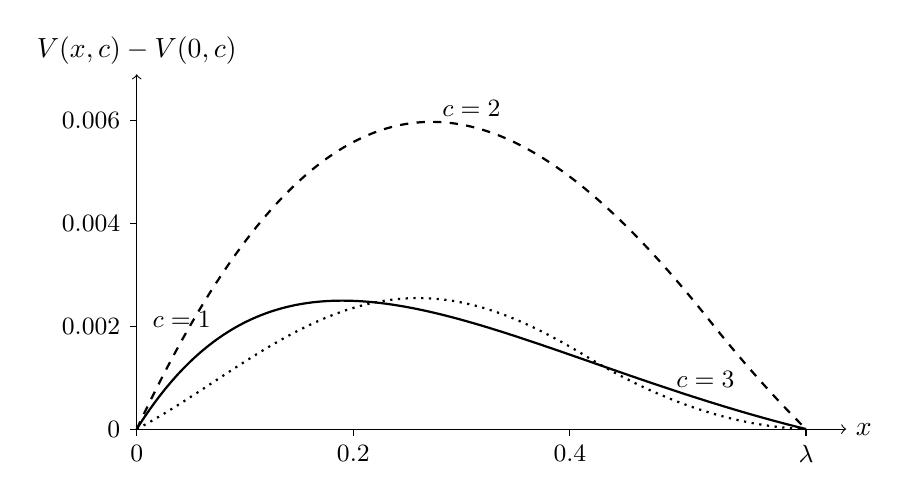
\begin{tikzpicture}[scale=0.85]
\draw[->] (0,0) -- (10.6,0) node[right] {$x$};
\draw[->] (0,0) -- (0,5.3) node[above] {$V(x,c)-V(0,c)$};
\draw (0.000,0) -- (0.000,-0.1) node[below, font=\small] {0};
\draw (3.236,0) -- (3.236,-0.1) node[below, font=\small] {0.2};
\draw (6.472,0) -- (6.472,-0.1) node[below, font=\small] {0.4};
\draw (10.000,0) -- (10.000,-0.1) node[below, font=\small] {$\lambda$};
\draw (0,0.000) -- (-0.1,0.000) node[left, font=\small] {0};
\draw (0,1.538) -- (-0.1,1.538) node[left, font=\small] {0.002};
\draw (0,3.077) -- (-0.1,3.077) node[left, font=\small] {0.004};
\draw (0,4.615) -- (-0.1,4.615) node[left, font=\small] {0.006};
\draw[thick, black] (0.0000,0.0000) -- (0.0417,0.0656) -- (0.0833,0.1295) -- (0.1250,0.1920) -- (0.1667,0.2529) -- (0.2083,0.3123) -- (0.2500,0.3702) -- (0.2917,0.4266) -- (0.3333,0.4817) -- (0.3750,0.5353) -- (0.4167,0.5876) -- (0.4583,0.6385) -- (0.5000,0.6880) -- (0.5417,0.7363) -- (0.5833,0.7833) -- (0.6250,0.8290) -- (0.6667,0.8735) -- (0.7083,0.9167) -- (0.7500,0.9587) -- (0.7917,0.9996) -- (0.8333,1.0393) -- (0.8750,1.0779) -- (0.9167,1.1153) -- (0.9583,1.1517) -- (1.0000,1.1869) -- (1.0417,1.2211) -- (1.0833,1.2543) -- (1.1250,1.2864) -- (1.1667,1.3176) -- (1.2083,1.3477) -- (1.2500,1.3769) -- (1.2917,1.4051) -- (1.3333,1.4324) -- (1.3750,1.4587) -- (1.4167,1.4842) -- (1.4583,1.5087) -- (1.5000,1.5324) -- (1.5417,1.5552) -- (1.5833,1.5772) -- (1.6250,1.5984) -- (1.6667,1.6187) -- (1.7083,1.6383) -- (1.7500,1.6570) -- (1.7917,1.6750) -- (1.8333,1.6922) -- (1.8750,1.7087) -- (1.9167,1.7245) -- (1.9583,1.7395) -- (2.0000,1.7539) -- (2.0417,1.7676) -- (2.0833,1.7805) -- (2.1250,1.7929) -- (2.1667,1.8045) -- (2.2083,1.8155) -- (2.2500,1.8259) -- (2.2917,1.8357) -- (2.3333,1.8449) -- (2.3750,1.8535) -- (2.4167,1.8615) -- (2.4583,1.8689) -- (2.5000,1.8758) -- (2.5417,1.8821) -- (2.5833,1.8879) -- (2.6250,1.8932) -- (2.6667,1.8979) -- (2.7083,1.9022) -- (2.7500,1.9059) -- (2.7917,1.9091) -- (2.8333,1.9119) -- (2.8750,1.9142) -- (2.9167,1.9160) -- (2.9583,1.9174) -- (3.0000,1.9184) -- (3.0417,1.9189) -- (3.0833,1.9190) -- (3.1250,1.9186) -- (3.1667,1.9179) -- (3.2083,1.9168) -- (3.2500,1.9152) -- (3.2917,1.9133) -- (3.3333,1.9111) -- (3.3750,1.9084) -- (3.4167,1.9054) -- (3.4583,1.9020) -- (3.5000,1.8983) -- (3.5417,1.8943) -- (3.5833,1.8899) -- (3.6250,1.8853) -- (3.6667,1.8802) -- (3.7083,1.8749) -- (3.7500,1.8693) -- (3.7917,1.8634) -- (3.8333,1.8572) -- (3.8750,1.8508) -- (3.9167,1.8440) -- (3.9583,1.8370) -- (4.0000,1.8297) -- (4.0417,1.8222) -- (4.0833,1.8144) -- (4.1250,1.8064) -- (4.1667,1.7981) -- (4.2083,1.7896) -- (4.2500,1.7809) -- (4.2917,1.7719) -- (4.3333,1.7628) -- (4.3750,1.7534) -- (4.4167,1.7438) -- (4.4583,1.7340) -- (4.5000,1.7241) -- (4.5417,1.7139) -- (4.5833,1.7036) -- (4.6250,1.6930) -- (4.6667,1.6823) -- (4.7083,1.6715) -- (4.7500,1.6604) -- (4.7917,1.6493) -- (4.8333,1.6379) -- (4.8750,1.6264) -- (4.9167,1.6148) -- (4.9583,1.6030) -- (5.0000,1.5911) -- (5.0417,1.5790) -- (5.0833,1.5668) -- (5.1250,1.5545) -- (5.1667,1.5421) -- (5.2083,1.5295) -- (5.2500,1.5169) -- (5.2917,1.5041) -- (5.3333,1.4912) -- (5.3750,1.4783) -- (5.4167,1.4652) -- (5.4583,1.4520) -- (5.5000,1.4388) -- (5.5417,1.4254) -- (5.5833,1.4120) -- (5.6250,1.3985) -- (5.6667,1.3849) -- (5.7083,1.3712) -- (5.7500,1.3575) -- (5.7917,1.3437) -- (5.8333,1.3299) -- (5.8750,1.3159) -- (5.9167,1.3020) -- (5.9583,1.2879) -- (6.0000,1.2739) -- (6.0417,1.2597) -- (6.0833,1.2455) -- (6.1250,1.2313) -- (6.1667,1.2171) -- (6.2083,1.2028) -- (6.2500,1.1884) -- (6.2917,1.1741) -- (6.3333,1.1597) -- (6.3750,1.1453) -- (6.4167,1.1308) -- (6.4583,1.1163) -- (6.5000,1.1019) -- (6.5417,1.0874) -- (6.5833,1.0728) -- (6.6250,1.0583) -- (6.6667,1.0438) -- (6.7083,1.0292) -- (6.7500,1.0147) -- (6.7917,1.0001) -- (6.8333,0.9856) -- (6.8750,0.9710) -- (6.9167,0.9565) -- (6.9583,0.9419) -- (7.0000,0.9274) -- (7.0417,0.9129) -- (7.0833,0.8984) -- (7.1250,0.8839) -- (7.1667,0.8694) -- (7.2083,0.8549) -- (7.2500,0.8405) -- (7.2917,0.8260) -- (7.3333,0.8116) -- (7.3750,0.7972) -- (7.4167,0.7829) -- (7.4583,0.7686) -- (7.5000,0.7543) -- (7.5417,0.7400) -- (7.5833,0.7258) -- (7.6250,0.7116) -- (7.6667,0.6974) -- (7.7083,0.6833) -- (7.7500,0.6692) -- (7.7917,0.6551) -- (7.8333,0.6411) -- (7.8750,0.6272) -- (7.9167,0.6133) -- (7.9583,0.5994) -- (8.0000,0.5856) -- (8.0417,0.5718) -- (8.0833,0.5581) -- (8.1250,0.5444) -- (8.1667,0.5308) -- (8.2083,0.5172) -- (8.2500,0.5037) -- (8.2917,0.4903) -- (8.3333,0.4769) -- (8.3750,0.4636) -- (8.4167,0.4503) -- (8.4583,0.4371) -- (8.5000,0.4239) -- (8.5417,0.4108) -- (8.5833,0.3978) -- (8.6250,0.3849) -- (8.6667,0.3720) -- (8.7083,0.3591) -- (8.7500,0.3464) -- (8.7917,0.3337) -- (8.8333,0.3211) -- (8.8750,0.3086) -- (8.9167,0.2961) -- (8.9583,0.2837) -- (9.0000,0.2714) -- (9.0417,0.2591) -- (9.0833,0.2470) -- (9.1250,0.2349) -- (9.1667,0.2228) -- (9.2083,0.2109) -- (9.2500,0.1991) -- (9.2917,0.1873) -- (9.3333,0.1756) -- (9.3750,0.1640) -- (9.4167,0.1524) -- (9.4583,0.1410) -- (9.5000,0.1296) -- (9.5417,0.1183) -- (9.5833,0.1071) -- (9.6250,0.0960) -- (9.6667,0.0850) -- (9.7083,0.0741) -- (9.7500,0.0632) -- (9.7917,0.0525) -- (9.8333,0.0418) -- (9.8750,0.0312) -- (9.9167,0.0207) -- (9.9583,0.0103) -- (10.0000,-0.0000);
\node[above left, font=\small] at (1.250,1.377) {$c=1$};
\draw[thick, black, dashed] (0.0000,0.0000) -- (0.0417,0.0884) -- (0.0833,0.1759) -- (0.1250,0.2626) -- (0.1667,0.3484) -- (0.2083,0.4334) -- (0.2500,0.5176) -- (0.2917,0.6009) -- (0.3333,0.6834) -- (0.3750,0.7650) -- (0.4167,0.8458) -- (0.4583,0.9257) -- (0.5000,1.0048) -- (0.5417,1.0830) -- (0.5833,1.1604) -- (0.6250,1.2368) -- (0.6667,1.3125) -- (0.7083,1.3872) -- (0.7500,1.4611) -- (0.7917,1.5341) -- (0.8333,1.6063) -- (0.8750,1.6775) -- (0.9167,1.7479) -- (0.9583,1.8174) -- (1.0000,1.8861) -- (1.0417,1.9539) -- (1.0833,2.0207) -- (1.1250,2.0868) -- (1.1667,2.1519) -- (1.2083,2.2162) -- (1.2500,2.2795) -- (1.2917,2.3420) -- (1.3333,2.4036) -- (1.3750,2.4644) -- (1.4167,2.5242) -- (1.4583,2.5832) -- (1.5000,2.6413) -- (1.5417,2.6985) -- (1.5833,2.7548) -- (1.6250,2.8103) -- (1.6667,2.8649) -- (1.7083,2.9185) -- (1.7500,2.9713) -- (1.7917,3.0233) -- (1.8333,3.0743) -- (1.8750,3.1245) -- (1.9167,3.1738) -- (1.9583,3.2222) -- (2.0000,3.2698) -- (2.0417,3.3164) -- (2.0833,3.3622) -- (2.1250,3.4071) -- (2.1667,3.4512) -- (2.2083,3.4944) -- (2.2500,3.5367) -- (2.2917,3.5781) -- (2.3333,3.6187) -- (2.3750,3.6584) -- (2.4167,3.6973) -- (2.4583,3.7353) -- (2.5000,3.7724) -- (2.5417,3.8087) -- (2.5833,3.8441) -- (2.6250,3.8787) -- (2.6667,3.9124) -- (2.7083,3.9452) -- (2.7500,3.9772) -- (2.7917,4.0084) -- (2.8333,4.0387) -- (2.8750,4.0682) -- (2.9167,4.0968) -- (2.9583,4.1246) -- (3.0000,4.1516) -- (3.0417,4.1777) -- (3.0833,4.2030) -- (3.1250,4.2275) -- (3.1667,4.2511) -- (3.2083,4.2740) -- (3.2500,4.2960) -- (3.2917,4.3171) -- (3.3333,4.3375) -- (3.3750,4.3570) -- (3.4167,4.3758) -- (3.4583,4.3937) -- (3.5000,4.4108) -- (3.5417,4.4272) -- (3.5833,4.4427) -- (3.6250,4.4574) -- (3.6667,4.4713) -- (3.7083,4.4845) -- (3.7500,4.4968) -- (3.7917,4.5084) -- (3.8333,4.5192) -- (3.8750,4.5292) -- (3.9167,4.5385) -- (3.9583,4.5469) -- (4.0000,4.5546) -- (4.0417,4.5616) -- (4.0833,4.5677) -- (4.1250,4.5731) -- (4.1667,4.5778) -- (4.2083,4.5817) -- (4.2500,4.5849) -- (4.2917,4.5873) -- (4.3333,4.5889) -- (4.3750,4.5899) -- (4.4167,4.5901) -- (4.4583,4.5895) -- (4.5000,4.5883) -- (4.5417,4.5863) -- (4.5833,4.5836) -- (4.6250,4.5802) -- (4.6667,4.5760) -- (4.7083,4.5712) -- (4.7500,4.5657) -- (4.7917,4.5594) -- (4.8333,4.5525) -- (4.8750,4.5448) -- (4.9167,4.5365) -- (4.9583,4.5275) -- (5.0000,4.5178) -- (5.0417,4.5074) -- (5.0833,4.4964) -- (5.1250,4.4847) -- (5.1667,4.4723) -- (5.2083,4.4592) -- (5.2500,4.4455) -- (5.2917,4.4312) -- (5.3333,4.4161) -- (5.3750,4.4005) -- (5.4167,4.3842) -- (5.4583,4.3673) -- (5.5000,4.3497) -- (5.5417,4.3315) -- (5.5833,4.3126) -- (5.6250,4.2932) -- (5.6667,4.2731) -- (5.7083,4.2524) -- (5.7500,4.2312) -- (5.7917,4.2093) -- (5.8333,4.1868) -- (5.8750,4.1637) -- (5.9167,4.1400) -- (5.9583,4.1157) -- (6.0000,4.0908) -- (6.0417,4.0654) -- (6.0833,4.0394) -- (6.1250,4.0128) -- (6.1667,3.9856) -- (6.2083,3.9579) -- (6.2500,3.9297) -- (6.2917,3.9008) -- (6.3333,3.8715) -- (6.3750,3.8415) -- (6.4167,3.8111) -- (6.4583,3.7801) -- (6.5000,3.7485) -- (6.5417,3.7165) -- (6.5833,3.6839) -- (6.6250,3.6508) -- (6.6667,3.6172) -- (6.7083,3.5830) -- (6.7500,3.5484) -- (6.7917,3.5132) -- (6.8333,3.4776) -- (6.8750,3.4415) -- (6.9167,3.4049) -- (6.9583,3.3678) -- (7.0000,3.3302) -- (7.0417,3.2921) -- (7.0833,3.2536) -- (7.1250,3.2146) -- (7.1667,3.1752) -- (7.2083,3.1352) -- (7.2500,3.0949) -- (7.2917,3.0541) -- (7.3333,3.0128) -- (7.3750,2.9711) -- (7.4167,2.9290) -- (7.4583,2.8864) -- (7.5000,2.8434) -- (7.5417,2.8000) -- (7.5833,2.7562) -- (7.6250,2.7120) -- (7.6667,2.6673) -- (7.7083,2.6223) -- (7.7500,2.5768) -- (7.7917,2.5310) -- (7.8333,2.4847) -- (7.8750,2.4381) -- (7.9167,2.3911) -- (7.9583,2.3437) -- (8.0000,2.2960) -- (8.0417,2.2478) -- (8.0833,2.1994) -- (8.1250,2.1505) -- (8.1667,2.1013) -- (8.2083,2.0518) -- (8.2500,2.0019) -- (8.2917,1.9516) -- (8.3333,1.9011) -- (8.3750,1.8502) -- (8.4167,1.7989) -- (8.4583,1.7474) -- (8.5000,1.6955) -- (8.5417,1.6433) -- (8.5833,1.5913) -- (8.6250,1.5394) -- (8.6667,1.4879) -- (8.7083,1.4366) -- (8.7500,1.3856) -- (8.7917,1.3348) -- (8.8333,1.2844) -- (8.8750,1.2342) -- (8.9167,1.1844) -- (8.9583,1.1348) -- (9.0000,1.0855) -- (9.0417,1.0365) -- (9.0833,0.9878) -- (9.1250,0.9395) -- (9.1667,0.8914) -- (9.2083,0.8437) -- (9.2500,0.7962) -- (9.2917,0.7491) -- (9.3333,0.7023) -- (9.3750,0.6559) -- (9.4167,0.6097) -- (9.4583,0.5639) -- (9.5000,0.5185) -- (9.5417,0.4733) -- (9.5833,0.4286) -- (9.6250,0.3841) -- (9.6667,0.3400) -- (9.7083,0.2963) -- (9.7500,0.2529) -- (9.7917,0.2098) -- (9.8333,0.1671) -- (9.8750,0.1248) -- (9.9167,0.0828) -- (9.9583,0.0412) -- (10.0000,0.0000);
\node[above, font=\small] at (5.000,4.518) {$c=2$};
\draw[thick, black, dotted] (0.0000,0.0000) -- (0.0417,0.0220) -- (0.0833,0.0444) -- (0.1250,0.0671) -- (0.1667,0.0902) -- (0.2083,0.1137) -- (0.2500,0.1375) -- (0.2917,0.1616) -- (0.3333,0.1861) -- (0.3750,0.2108) -- (0.4167,0.2358) -- (0.4583,0.2610) -- (0.5000,0.2866) -- (0.5417,0.3123) -- (0.5833,0.3383) -- (0.6250,0.3644) -- (0.6667,0.3908) -- (0.7083,0.4173) -- (0.7500,0.4440) -- (0.7917,0.4708) -- (0.8333,0.4977) -- (0.8750,0.5248) -- (0.9167,0.5519) -- (0.9583,0.5792) -- (1.0000,0.6065) -- (1.0417,0.6338) -- (1.0833,0.6612) -- (1.1250,0.6886) -- (1.1667,0.7160) -- (1.2083,0.7434) -- (1.2500,0.7708) -- (1.2917,0.7981) -- (1.3333,0.8254) -- (1.3750,0.8527) -- (1.4167,0.8798) -- (1.4583,0.9069) -- (1.5000,0.9338) -- (1.5417,0.9606) -- (1.5833,0.9873) -- (1.6250,1.0139) -- (1.6667,1.0402) -- (1.7083,1.0664) -- (1.7500,1.0925) -- (1.7917,1.1183) -- (1.8333,1.1439) -- (1.8750,1.1693) -- (1.9167,1.1944) -- (1.9583,1.2193) -- (2.0000,1.2440) -- (2.0417,1.2683) -- (2.0833,1.2924) -- (2.1250,1.3162) -- (2.1667,1.3397) -- (2.2083,1.3629) -- (2.2500,1.3858) -- (2.2917,1.4083) -- (2.3333,1.4305) -- (2.3750,1.4523) -- (2.4167,1.4738) -- (2.4583,1.4948) -- (2.5000,1.5156) -- (2.5417,1.5359) -- (2.5833,1.5558) -- (2.6250,1.5753) -- (2.6667,1.5944) -- (2.7083,1.6131) -- (2.7500,1.6313) -- (2.7917,1.6491) -- (2.8333,1.6665) -- (2.8750,1.6834) -- (2.9167,1.6999) -- (2.9583,1.7159) -- (3.0000,1.7314) -- (3.0417,1.7464) -- (3.0833,1.7610) -- (3.1250,1.7751) -- (3.1667,1.7886) -- (3.2083,1.8017) -- (3.2500,1.8143) -- (3.2917,1.8264) -- (3.3333,1.8379) -- (3.3750,1.8490) -- (3.4167,1.8595) -- (3.4583,1.8695) -- (3.5000,1.8790) -- (3.5417,1.8879) -- (3.5833,1.8963) -- (3.6250,1.9042) -- (3.6667,1.9116) -- (3.7083,1.9184) -- (3.7500,1.9246) -- (3.7917,1.9303) -- (3.8333,1.9355) -- (3.8750,1.9401) -- (3.9167,1.9442) -- (3.9583,1.9477) -- (4.0000,1.9507) -- (4.0417,1.9531) -- (4.0833,1.9549) -- (4.1250,1.9563) -- (4.1667,1.9570) -- (4.2083,1.9573) -- (4.2500,1.9569) -- (4.2917,1.9560) -- (4.3333,1.9546) -- (4.3750,1.9526) -- (4.4167,1.9501) -- (4.4583,1.9470) -- (4.5000,1.9434) -- (4.5417,1.9393) -- (4.5833,1.9346) -- (4.6250,1.9294) -- (4.6667,1.9236) -- (4.7083,1.9174) -- (4.7500,1.9105) -- (4.7917,1.9032) -- (4.8333,1.8954) -- (4.8750,1.8870) -- (4.9167,1.8781) -- (4.9583,1.8687) -- (5.0000,1.8588) -- (5.0417,1.8484) -- (5.0833,1.8375) -- (5.1250,1.8261) -- (5.1667,1.8143) -- (5.2083,1.8019) -- (5.2500,1.7891) -- (5.2917,1.7758) -- (5.3333,1.7620) -- (5.3750,1.7478) -- (5.4167,1.7331) -- (5.4583,1.7179) -- (5.5000,1.7024) -- (5.5417,1.6863) -- (5.5833,1.6699) -- (5.6250,1.6530) -- (5.6667,1.6358) -- (5.7083,1.6181) -- (5.7500,1.6000) -- (5.7917,1.5815) -- (5.8333,1.5626) -- (5.8750,1.5434) -- (5.9167,1.5237) -- (5.9583,1.5038) -- (6.0000,1.4834) -- (6.0417,1.4627) -- (6.0833,1.4417) -- (6.1250,1.4203) -- (6.1667,1.3986) -- (6.2083,1.3766) -- (6.2500,1.3543) -- (6.2917,1.3317) -- (6.3333,1.3089) -- (6.3750,1.2857) -- (6.4167,1.2623) -- (6.4583,1.2386) -- (6.5000,1.2146) -- (6.5417,1.1905) -- (6.5833,1.1661) -- (6.6250,1.1414) -- (6.6667,1.1166) -- (6.7083,1.0916) -- (6.7500,1.0664) -- (6.7917,1.0414) -- (6.8333,1.0168) -- (6.8750,0.9924) -- (6.9167,0.9683) -- (6.9583,0.9444) -- (7.0000,0.9209) -- (7.0417,0.8976) -- (7.0833,0.8746) -- (7.1250,0.8519) -- (7.1667,0.8295) -- (7.2083,0.8073) -- (7.2500,0.7855) -- (7.2917,0.7639) -- (7.3333,0.7426) -- (7.3750,0.7216) -- (7.4167,0.7009) -- (7.4583,0.6804) -- (7.5000,0.6603) -- (7.5417,0.6404) -- (7.5833,0.6208) -- (7.6250,0.6015) -- (7.6667,0.5825) -- (7.7083,0.5638) -- (7.7500,0.5454) -- (7.7917,0.5272) -- (7.8333,0.5094) -- (7.8750,0.4918) -- (7.9167,0.4746) -- (7.9583,0.4576) -- (8.0000,0.4409) -- (8.0417,0.4245) -- (8.0833,0.4085) -- (8.1250,0.3927) -- (8.1667,0.3772) -- (8.2083,0.3620) -- (8.2500,0.3471) -- (8.2917,0.3324) -- (8.3333,0.3181) -- (8.3750,0.3041) -- (8.4167,0.2904) -- (8.4583,0.2770) -- (8.5000,0.2639) -- (8.5417,0.2511) -- (8.5833,0.2386) -- (8.6250,0.2264) -- (8.6667,0.2145) -- (8.7083,0.2029) -- (8.7500,0.1916) -- (8.7917,0.1806) -- (8.8333,0.1700) -- (8.8750,0.1596) -- (8.9167,0.1496) -- (8.9583,0.1398) -- (9.0000,0.1304) -- (9.0417,0.1213) -- (9.0833,0.1125) -- (9.1250,0.1040) -- (9.1667,0.0958) -- (9.2083,0.0879) -- (9.2500,0.0804) -- (9.2917,0.0732) -- (9.3333,0.0663) -- (9.3750,0.0597) -- (9.4167,0.0534) -- (9.4583,0.0475) -- (9.5000,0.0419) -- (9.5417,0.0366) -- (9.5833,0.0316) -- (9.6250,0.0270) -- (9.6667,0.0226) -- (9.7083,0.0187) -- (9.7500,0.0150) -- (9.7917,0.0117) -- (9.8333,0.0087) -- (9.8750,0.0060) -- (9.9167,0.0037) -- (9.9583,0.0017) -- (10.0000,-0.0000);
\node[above right, font=\small] at (7.917,0.475) {$c=3$};

\end{tikzpicture}
\caption{Golden angle: excess $V(x,c)-V(0,c)$ of the subsequential limit along
$N=F_m+\lfloor xF_m\rfloor$ over the Fibonacci limit, for $c=1$ (solid), $2$ (dashed), $3$
(dotted). Nonnegativity is the convex-order statement of Theorem~\ref{thm:B}.}
\label{fig:phase}
\end{figure}

\begin{figure}[t]
\centering
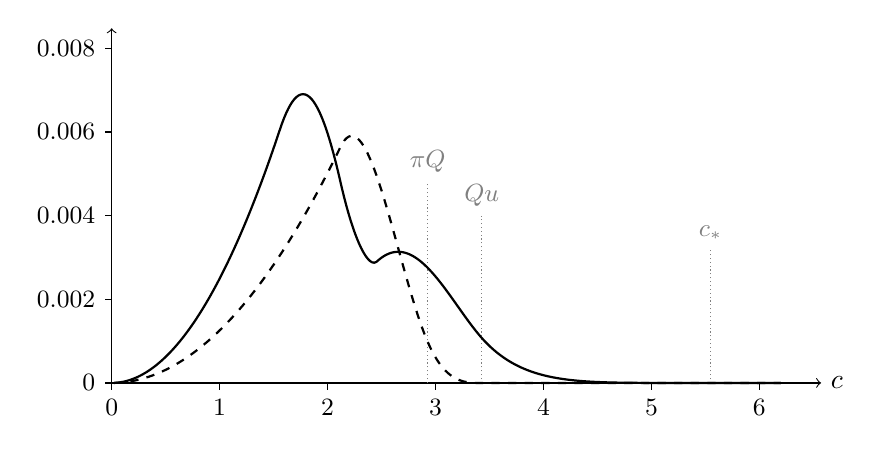
\begin{tikzpicture}[scale=0.85]
\draw[->] (0,0) -- (10.6,0) node[right] {$c$};
\draw[->] (0,0) -- (0,5.3);
\draw (0.000,0) -- (0.000,-0.1) node[below, font=\small] {0};
\draw (1.613,0) -- (1.613,-0.1) node[below, font=\small] {1};
\draw (3.226,0) -- (3.226,-0.1) node[below, font=\small] {2};
\draw (4.839,0) -- (4.839,-0.1) node[below, font=\small] {3};
\draw (6.452,0) -- (6.452,-0.1) node[below, font=\small] {4};
\draw (8.065,0) -- (8.065,-0.1) node[below, font=\small] {5};
\draw (9.677,0) -- (9.677,-0.1) node[below, font=\small] {6};
\draw (0,0.000) -- (-0.1,0.000) node[left, font=\small] {0};
\draw (0,1.250) -- (-0.1,1.250) node[left, font=\small] {0.002};
\draw (0,2.500) -- (-0.1,2.500) node[left, font=\small] {0.004};
\draw (0,3.750) -- (-0.1,3.750) node[left, font=\small] {0.006};
\draw (0,5.000) -- (-0.1,5.000) node[left, font=\small] {0.008};
\draw[gray, densely dotted] (8.947,0) -- (8.947,2) node[above, font=\small] {$c_*$};
\draw[gray, densely dotted] (4.723,0) -- (4.723,3) node[above, font=\small] {$\pi Q$};
\draw[gray, densely dotted] (5.529,0) -- (5.529,2.5) node[above, font=\small] {$Qu$};
\draw[thick, black] (0.0323,0.0006) -- (0.0644,0.0025) -- (0.0966,0.0056) -- (0.1287,0.0099) -- (0.1609,0.0155) -- (0.1930,0.0223) -- (0.2252,0.0304) -- (0.2573,0.0397) -- (0.2895,0.0502) -- (0.3216,0.0620) -- (0.3538,0.0750) -- (0.3860,0.0893) -- (0.4181,0.1048) -- (0.4503,0.1215) -- (0.4824,0.1395) -- (0.5146,0.1587) -- (0.5467,0.1791) -- (0.5789,0.2008) -- (0.6110,0.2238) -- (0.6432,0.2479) -- (0.6753,0.2733) -- (0.7075,0.3000) -- (0.7396,0.3279) -- (0.7718,0.3570) -- (0.8040,0.3874) -- (0.8361,0.4190) -- (0.8683,0.4518) -- (0.9004,0.4859) -- (0.9326,0.5212) -- (0.9647,0.5578) -- (0.9969,0.5956) -- (1.0290,0.6346) -- (1.0612,0.6749) -- (1.0933,0.7164) -- (1.1255,0.7592) -- (1.1576,0.8032) -- (1.1898,0.8484) -- (1.2220,0.8949) -- (1.2541,0.9426) -- (1.2863,0.9916) -- (1.3184,1.0418) -- (1.3506,1.0932) -- (1.3827,1.1459) -- (1.4149,1.1998) -- (1.4470,1.2550) -- (1.4792,1.3114) -- (1.5113,1.3690) -- (1.5435,1.4279) -- (1.5757,1.4880) -- (1.6078,1.5493) -- (1.6400,1.6119) -- (1.6721,1.6757) -- (1.7043,1.7408) -- (1.7364,1.8071) -- (1.7686,1.8746) -- (1.8007,1.9434) -- (1.8329,2.0135) -- (1.8650,2.0847) -- (1.8972,2.1572) -- (1.9293,2.2310) -- (1.9615,2.3059) -- (1.9937,2.3822) -- (2.0258,2.4596) -- (2.0580,2.5383) -- (2.0901,2.6183) -- (2.1223,2.6994) -- (2.1544,2.7819) -- (2.1866,2.8655) -- (2.2187,2.9504) -- (2.2509,3.0365) -- (2.2830,3.1239) -- (2.3152,3.2125) -- (2.3473,3.3024) -- (2.3795,3.3935) -- (2.4117,3.4858) -- (2.4438,3.5794) -- (2.4760,3.6742) -- (2.5081,3.7702) -- (2.5403,3.8639) -- (2.5724,3.9493) -- (2.6046,4.0260) -- (2.6367,4.0941) -- (2.6689,4.1534) -- (2.7010,4.2035) -- (2.7332,4.2444) -- (2.7653,4.2759) -- (2.7975,4.2980) -- (2.8297,4.3108) -- (2.8618,4.3148) -- (2.8940,4.3092) -- (2.9261,4.2942) -- (2.9583,4.2702) -- (2.9904,4.2372) -- (3.0226,4.1948) -- (3.0547,4.1440) -- (3.0869,4.0842) -- (3.1190,4.0158) -- (3.1512,3.9391) -- (3.1834,3.8539) -- (3.2155,3.7609) -- (3.2477,3.6600) -- (3.2798,3.5512) -- (3.3120,3.4354) -- (3.3441,3.3124) -- (3.3763,3.1824) -- (3.4084,3.0459) -- (3.4406,2.9070) -- (3.4727,2.7759) -- (3.5049,2.6530) -- (3.5370,2.5381) -- (3.5692,2.4310) -- (3.6014,2.3316) -- (3.6335,2.2397) -- (3.6657,2.1555) -- (3.6978,2.0791) -- (3.7300,2.0105) -- (3.7621,1.9499) -- (3.7943,1.8980) -- (3.8264,1.8554) -- (3.8586,1.8231) -- (3.8907,1.8026) -- (3.9229,1.7964) -- (3.9550,1.8089) -- (3.9872,1.8364) -- (4.0194,1.8623) -- (4.0515,1.8850) -- (4.0837,1.9046) -- (4.1158,1.9209) -- (4.1480,1.9347) -- (4.1801,1.9455) -- (4.2123,1.9531) -- (4.2444,1.9576) -- (4.2766,1.9597) -- (4.3087,1.9588) -- (4.3409,1.9549) -- (4.3730,1.9482) -- (4.4052,1.9392) -- (4.4374,1.9273) -- (4.4695,1.9126) -- (4.5017,1.8958) -- (4.5338,1.8765) -- (4.5660,1.8547) -- (4.5981,1.8308) -- (4.6303,1.8048) -- (4.6624,1.7765) -- (4.6946,1.7463) -- (4.7267,1.7145) -- (4.7589,1.6808) -- (4.7911,1.6453) -- (4.8232,1.6086) -- (4.8554,1.5702) -- (4.8875,1.5305) -- (4.9197,1.4899) -- (4.9518,1.4481) -- (4.9840,1.4052) -- (5.0161,1.3618) -- (5.0483,1.3176) -- (5.0804,1.2728) -- (5.1126,1.2278) -- (5.1447,1.1824) -- (5.1769,1.1369) -- (5.2091,1.0915) -- (5.2412,1.0462) -- (5.2734,1.0012) -- (5.3055,0.9568) -- (5.3377,0.9128) -- (5.3698,0.8698) -- (5.4020,0.8276) -- (5.4341,0.7863) -- (5.4663,0.7465) -- (5.4984,0.7079) -- (5.5306,0.6709) -- (5.5627,0.6355) -- (5.5949,0.6017) -- (5.6271,0.5695) -- (5.6592,0.5388) -- (5.6914,0.5094) -- (5.7235,0.4816) -- (5.7557,0.4549) -- (5.7878,0.4296) -- (5.8200,0.4054) -- (5.8521,0.3824) -- (5.8843,0.3606) -- (5.9164,0.3398) -- (5.9486,0.3201) -- (5.9807,0.3013) -- (6.0129,0.2834) -- (6.0451,0.2665) -- (6.0772,0.2504) -- (6.1094,0.2352) -- (6.1415,0.2207) -- (6.1737,0.2071) -- (6.2058,0.1941) -- (6.2380,0.1818) -- (6.2701,0.1702) -- (6.3023,0.1592) -- (6.3344,0.1488) -- (6.3666,0.1390) -- (6.3988,0.1298) -- (6.4309,0.1210) -- (6.4631,0.1128) -- (6.4952,0.1050) -- (6.5274,0.0977) -- (6.5595,0.0908) -- (6.5917,0.0843) -- (6.6238,0.0783) -- (6.6560,0.0726) -- (6.6881,0.0672) -- (6.7203,0.0622) -- (6.7524,0.0575) -- (6.7846,0.0531) -- (6.8168,0.0489) -- (6.8489,0.0451) -- (6.8811,0.0415) -- (6.9132,0.0381) -- (6.9454,0.0350) -- (6.9775,0.0321) -- (7.0097,0.0294) -- (7.0418,0.0269) -- (7.0740,0.0245) -- (7.1061,0.0224) -- (7.1383,0.0204) -- (7.1704,0.0185) -- (7.2026,0.0168) -- (7.2348,0.0152) -- (7.2669,0.0138) -- (7.2991,0.0124) -- (7.3312,0.0112) -- (7.3634,0.0101) -- (7.3955,0.0090) -- (7.4277,0.0081) -- (7.4598,0.0072) -- (7.4920,0.0064) -- (7.5241,0.0057) -- (7.5563,0.0051) -- (7.5884,0.0045) -- (7.6206,0.0040) -- (7.6528,0.0035) -- (7.6849,0.0031) -- (7.7171,0.0027) -- (7.7492,0.0023) -- (7.7814,0.0020) -- (7.8135,0.0018) -- (7.8457,0.0015) -- (7.8778,0.0013) -- (7.9100,0.0011) -- (7.9421,0.0009) -- (7.9743,0.0008) -- (8.0065,0.0007) -- (8.0386,0.0006) -- (8.0708,0.0005) -- (8.1029,0.0004) -- (8.1351,0.0003) -- (8.1672,0.0003) -- (8.1994,0.0002) -- (8.2315,0.0002) -- (8.2637,0.0001) -- (8.2958,0.0001) -- (8.3280,0.0001) -- (8.3601,0.0001) -- (8.3923,0.0000) -- (8.4245,0.0000) -- (8.4566,0.0000) -- (8.4888,0.0000) -- (8.5209,0.0000) -- (8.5531,0.0000) -- (8.5852,0.0000) -- (8.6174,0.0000) -- (8.6495,0.0000) -- (8.6817,0.0000) -- (8.7138,0.0000) -- (8.7460,0.0000) -- (8.7781,0.0000) -- (8.8103,0.0000) -- (8.8425,0.0000) -- (8.8746,0.0000) -- (8.9068,0.0000) -- (8.9389,0.0000) -- (8.9711,0.0000) -- (9.0032,0.0000) -- (9.0354,0.0000) -- (9.0675,0.0000) -- (9.0997,0.0000) -- (9.1318,0.0000) -- (9.1640,0.0000) -- (9.1961,0.0000) -- (9.2283,0.0000) -- (9.2605,0.0000) -- (9.2926,0.0000) -- (9.3248,0.0000) -- (9.3569,0.0000) -- (9.3891,0.0000) -- (9.4212,0.0000) -- (9.4534,0.0000) -- (9.4855,0.0000) -- (9.5177,0.0000) -- (9.5498,0.0000) -- (9.5820,0.0000) -- (9.6142,0.0000) -- (9.6463,0.0000) -- (9.6785,0.0000) -- (9.7106,0.0000) -- (9.7428,0.0000) -- (9.7749,0.0000) -- (9.8071,0.0000) -- (9.8392,0.0000) -- (9.8714,0.0000) -- (9.9035,0.0000) -- (9.9357,0.0000) -- (9.9678,0.0000) -- (10.0000,0.0000);
\draw[thick, black, dashed] (0.0323,0.0003) -- (0.0644,0.0013) -- (0.0966,0.0028) -- (0.1287,0.0050) -- (0.1609,0.0078) -- (0.1930,0.0112) -- (0.2252,0.0153) -- (0.2573,0.0200) -- (0.2895,0.0253) -- (0.3216,0.0312) -- (0.3538,0.0378) -- (0.3860,0.0449) -- (0.4181,0.0527) -- (0.4503,0.0612) -- (0.4824,0.0702) -- (0.5146,0.0799) -- (0.5467,0.0902) -- (0.5789,0.1011) -- (0.6110,0.1127) -- (0.6432,0.1248) -- (0.6753,0.1376) -- (0.7075,0.1510) -- (0.7396,0.1651) -- (0.7718,0.1797) -- (0.8040,0.1950) -- (0.8361,0.2109) -- (0.8683,0.2275) -- (0.9004,0.2446) -- (0.9326,0.2624) -- (0.9647,0.2808) -- (0.9969,0.2998) -- (1.0290,0.3195) -- (1.0612,0.3398) -- (1.0933,0.3607) -- (1.1255,0.3822) -- (1.1576,0.4044) -- (1.1898,0.4271) -- (1.2220,0.4505) -- (1.2541,0.4745) -- (1.2863,0.4992) -- (1.3184,0.5245) -- (1.3506,0.5504) -- (1.3827,0.5769) -- (1.4149,0.6040) -- (1.4470,0.6318) -- (1.4792,0.6602) -- (1.5113,0.6892) -- (1.5435,0.7188) -- (1.5757,0.7491) -- (1.6078,0.7800) -- (1.6400,0.8115) -- (1.6721,0.8436) -- (1.7043,0.8764) -- (1.7364,0.9097) -- (1.7686,0.9437) -- (1.8007,0.9784) -- (1.8329,1.0136) -- (1.8650,1.0495) -- (1.8972,1.0860) -- (1.9293,1.1231) -- (1.9615,1.1609) -- (1.9937,1.1992) -- (2.0258,1.2382) -- (2.0580,1.2779) -- (2.0901,1.3181) -- (2.1223,1.3590) -- (2.1544,1.4005) -- (2.1866,1.4426) -- (2.2187,1.4853) -- (2.2509,1.5287) -- (2.2830,1.5727) -- (2.3152,1.6173) -- (2.3473,1.6625) -- (2.3795,1.7084) -- (2.4117,1.7548) -- (2.4438,1.8019) -- (2.4760,1.8497) -- (2.5081,1.8980) -- (2.5403,1.9470) -- (2.5724,1.9966) -- (2.6046,2.0468) -- (2.6367,2.0977) -- (2.6689,2.1492) -- (2.7010,2.2013) -- (2.7332,2.2540) -- (2.7653,2.3073) -- (2.7975,2.3613) -- (2.8297,2.4159) -- (2.8618,2.4711) -- (2.8940,2.5269) -- (2.9261,2.5834) -- (2.9583,2.6405) -- (2.9904,2.6982) -- (3.0226,2.7565) -- (3.0547,2.8155) -- (3.0869,2.8751) -- (3.1190,2.9353) -- (3.1512,2.9961) -- (3.1834,3.0576) -- (3.2155,3.1197) -- (3.2477,3.1824) -- (3.2798,3.2457) -- (3.3120,3.3096) -- (3.3441,3.3742) -- (3.3763,3.4394) -- (3.4084,3.5052) -- (3.4406,3.5679) -- (3.4727,3.6175) -- (3.5049,3.6540) -- (3.5370,3.6780) -- (3.5692,3.6901) -- (3.6014,3.6909) -- (3.6335,3.6808) -- (3.6657,3.6605) -- (3.6978,3.6305) -- (3.7300,3.5913) -- (3.7621,3.5436) -- (3.7943,3.4877) -- (3.8264,3.4243) -- (3.8586,3.3538) -- (3.8907,3.2769) -- (3.9229,3.1939) -- (3.9550,3.1055) -- (3.9872,3.0121) -- (4.0194,2.9142) -- (4.0515,2.8124) -- (4.0837,2.7071) -- (4.1158,2.5988) -- (4.1480,2.4880) -- (4.1801,2.3752) -- (4.2123,2.2609) -- (4.2444,2.1455) -- (4.2766,2.0295) -- (4.3087,1.9135) -- (4.3409,1.7978) -- (4.3730,1.6829) -- (4.4052,1.5693) -- (4.4374,1.4574) -- (4.4695,1.3477) -- (4.5017,1.2406) -- (4.5338,1.1367) -- (4.5660,1.0362) -- (4.5981,0.9397) -- (4.6303,0.8476) -- (4.6624,0.7604) -- (4.6946,0.6784) -- (4.7267,0.6021) -- (4.7589,0.5318) -- (4.7911,0.4672) -- (4.8232,0.4081) -- (4.8554,0.3543) -- (4.8875,0.3055) -- (4.9197,0.2615) -- (4.9518,0.2219) -- (4.9840,0.1866) -- (5.0161,0.1553) -- (5.0483,0.1277) -- (5.0804,0.1036) -- (5.1126,0.0828) -- (5.1447,0.0650) -- (5.1769,0.0499) -- (5.2091,0.0374) -- (5.2412,0.0272) -- (5.2734,0.0190) -- (5.3055,0.0127) -- (5.3377,0.0080) -- (5.3698,0.0046) -- (5.4020,0.0023) -- (5.4341,0.0010) -- (5.4663,0.0003) -- (5.4984,0.0000) -- (5.5306,0.0000) -- (5.5627,0.0000) -- (5.5949,0.0000) -- (5.6271,0.0000) -- (5.6592,0.0000) -- (5.6914,0.0000) -- (5.7235,0.0000) -- (5.7557,0.0000) -- (5.7878,0.0000) -- (5.8200,0.0000) -- (5.8521,0.0000) -- (5.8843,0.0000) -- (5.9164,0.0000) -- (5.9486,0.0000) -- (5.9807,0.0000) -- (6.0129,0.0000) -- (6.0451,0.0000) -- (6.0772,0.0000) -- (6.1094,0.0000) -- (6.1415,0.0000) -- (6.1737,0.0000) -- (6.2058,0.0000) -- (6.2380,0.0000) -- (6.2701,0.0000) -- (6.3023,0.0000) -- (6.3344,0.0000) -- (6.3666,0.0000) -- (6.3988,0.0000) -- (6.4309,0.0000) -- (6.4631,0.0000) -- (6.4952,0.0000) -- (6.5274,0.0000) -- (6.5595,0.0000) -- (6.5917,0.0000) -- (6.6238,0.0000) -- (6.6560,0.0000) -- (6.6881,0.0000) -- (6.7203,0.0000) -- (6.7524,0.0000) -- (6.7846,0.0000) -- (6.8168,0.0000) -- (6.8489,0.0000) -- (6.8811,0.0000) -- (6.9132,0.0000) -- (6.9454,0.0000) -- (6.9775,0.0000) -- (7.0097,0.0000) -- (7.0418,0.0000) -- (7.0740,0.0000) -- (7.1061,0.0000) -- (7.1383,0.0000) -- (7.1704,0.0000) -- (7.2026,0.0000) -- (7.2348,0.0000) -- (7.2669,0.0000) -- (7.2991,0.0000) -- (7.3312,0.0000) -- (7.3634,0.0000) -- (7.3955,0.0000) -- (7.4277,0.0000) -- (7.4598,0.0000) -- (7.4920,0.0000) -- (7.5241,0.0000) -- (7.5563,0.0000) -- (7.5884,0.0000) -- (7.6206,0.0000) -- (7.6528,0.0000) -- (7.6849,0.0000) -- (7.7171,0.0000) -- (7.7492,0.0000) -- (7.7814,0.0000) -- (7.8135,0.0000) -- (7.8457,0.0000) -- (7.8778,0.0000) -- (7.9100,0.0000) -- (7.9421,0.0000) -- (7.9743,0.0000) -- (8.0065,0.0000) -- (8.0386,0.0000) -- (8.0708,0.0000) -- (8.1029,0.0000) -- (8.1351,0.0000) -- (8.1672,0.0000) -- (8.1994,0.0000) -- (8.2315,0.0000) -- (8.2637,0.0000) -- (8.2958,0.0000) -- (8.3280,0.0000) -- (8.3601,0.0000) -- (8.3923,0.0000) -- (8.4245,0.0000) -- (8.4566,0.0000) -- (8.4888,0.0000) -- (8.5209,0.0000) -- (8.5531,0.0000) -- (8.5852,0.0000) -- (8.6174,0.0000) -- (8.6495,0.0000) -- (8.6817,0.0000) -- (8.7138,0.0000) -- (8.7460,0.0000) -- (8.7781,0.0000) -- (8.8103,0.0000) -- (8.8425,0.0000) -- (8.8746,0.0000) -- (8.9068,0.0000) -- (8.9389,0.0000) -- (8.9711,0.0000) -- (9.0032,0.0000) -- (9.0354,0.0000) -- (9.0675,0.0000) -- (9.0997,0.0000) -- (9.1318,0.0000) -- (9.1640,0.0000) -- (9.1961,0.0000) -- (9.2283,0.0000) -- (9.2605,0.0000) -- (9.2926,0.0000) -- (9.3248,0.0000) -- (9.3569,0.0000) -- (9.3891,0.0000) -- (9.4212,0.0000) -- (9.4534,0.0000) -- (9.4855,0.0000) -- (9.5177,0.0000) -- (9.5498,0.0000) -- (9.5820,0.0000) -- (9.6142,0.0000) -- (9.6463,0.0000) -- (9.6785,0.0000) -- (9.7106,0.0000) -- (9.7428,0.0000) -- (9.7749,0.0000) -- (9.8071,0.0000) -- (9.8392,0.0000) -- (9.8714,0.0000) -- (9.9035,0.0000) -- (9.9357,0.0000) -- (9.9678,0.0000) -- (10.0000,0.0000);

\end{tikzpicture}
\caption{Golden angle. Solid: oscillation amplitude $\limsup V_N(c)-\liminf V_N(c)=\max_xV(x,c)-V(0,c)$, positive exactly for $c<c_*$. Dashed: $\liminf V_N(c)-\Vd(c)=V(0,c)-\Vd(c)$, positive for $c<\pi Q$ as in Theorem~\ref{thm:C}(3).}
\label{fig:threshold}
\end{figure}

\paragraph{Certified constants.}
Interval arithmetic at 50 significant digits (\texttt{mpmath.iv}) applied to the
piecewise primitive $A^2q^2-4ABq+2B^2\log q$ of $2q(A-B/q)^2$ (on each interval of active
gap classes, $A=\sum f_i\ell_i/\pi$, $B=c\sum f_i/\pi$) gives the enclosures in
Table~\ref{tab:limits}. Strict inequality of the limits is already proved above; the
intervals only certify digits.

\begin{table}[t]
\centering
\begin{tabular}{@{}lll@{}}
\toprule
& $c=1$ & $c=2$\\
\midrule
$V(0,c)$ & $0.33622612952297228671\ldots$ & $0.15646165385915441214\ldots$\\
$V(1/3,c)$ & $0.33814037172223894875\ldots$ & $0.16217301017105651466\ldots$\\
difference & $0.00191424219926666204\ldots$ & $0.00571135631190210251\ldots$\\
\bottomrule
\end{tabular}
\caption{Certified golden-angle limits; also $a^2=0.13131556096084004924\ldots$ and
$c_*=5.54700825580342652455\ldots$.}
\label{tab:limits}
\end{table}

\section{Numerical experiments}\label{sec:numerics}

\paragraph{Monte Carlo.} Four million points uniform in $D$ (NumPy PCG64, seed
20261115) were tested against the true finite segments for $N=4181=F_{19}$ and
$N=5574=F_{19}+\lfloor F_{19}/3\rfloor$, using a four-candidate reduction whose
completeness we prove in the repository (distance to finitely many chords is minimized
by an angular neighbour of one of two continuous minimizers). Common random numbers
give paired standard errors.

\begin{center}
\begin{tabular}{@{}lllll@{}}
\toprule
$c$ & $V_{4181}$ & $V_{5574}$ & paired difference (SE) & limit difference\\
\midrule
1 & 0.33615200 & 0.33818425 & 0.00203225 (0.00019131) & 0.00191424\\
2 & 0.15617325 & 0.16190950 & 0.00573625 (0.00010177) & 0.00571136\\
\bottomrule
\end{tabular}
\end{center}

Across 20 independent seeds (16 further seeds 9001--9016 and three of an independent
verifier), the pooled $z$-scores of the paired differences against the deterministic
finite-$N$ values below are $0.91$ ($c=1$) and $1.43$ ($c=2$), and the spread across runs
matches the paired standard error.

\paragraph{Deterministic integration.} An independently written integrator computes, for
each radius $r$, the exact angular measure of the union of the covered arcs (interior
projection arcs and endpoint arcs of every finite chord, merged exactly) and integrates
$2rU_N(r)$ by composite Gauss--Legendre quadrature with breakpoints at $a\pm w$, $a$ and the
endpoint radii; halving the panel width changes $V_N$ by at most $2.4\times10^{-6}$ at
$N\approx4000$. Per-chord arcs agreed with dense brute angular sampling at every test point.
Selected values at $c=1$:
\begin{center}
\begin{tabular}{@{}rrllrrll@{}}
\toprule
\multicolumn{4}{c}{$x=0$ ($N=F_m$)} & \multicolumn{4}{c}{$x\approx1/3$}\\
$m$ & $N$ & $V_N$ & $N(V_N-V(0,1))$ & $m$ & $N$ & $V_N$ & $N(V_N-V(\tfrac13,1))$\\
\midrule
15 & 610 & 0.335072 & $-0.70$ & 15 & 813 & 0.337250 & $-0.73$\\
18 & 2584 & 0.335951 & $-0.71$ & 18 & 3445 & 0.337932 & $-0.72$\\
21 & 10946 & 0.336159 & $-0.74$ & 21 & 14594 & 0.338095 & $-0.67$\\
\bottomrule
\end{tabular}
\end{center}
For $m=12,\dots,21$ and $c\in\{0.5,1,2,3\}$ the log--log slope of $|V_N-V(x_N,c)|$ against
$N$ lies between $-0.93$ and $-1.01$. The offset at $c=1$ is close to $-2ac/N\approx-0.725/N$,
the deficit of the caustic disk of radius $a-c/N$; at these $N$, $\tilde V_N$ agrees with
$V(x,c)$ to six digits, so the error is dominated by geometry, not arithmetic. Within the
Fibonacci blocks $m=20,21$ ($15$--$17$ phases each, $c=1,2$), the smallest $V_N$ occurs at
$x=0$, as Theorem~\ref{thm:B} predicts. Near the threshold, after adding back $2ac/N$, the
excess over $a^2$ at $m=20$ is $5.99\times10^{-5}$ for $c=4$, $x=0.55$ (limit
$5.93\times10^{-5}$); for $c\ge5.4$ the predicted excess is below $10^{-9}$ and is not
resolvable at $N\approx10^4$, so the numerics support the shape of the threshold, not its
exact location. These are double-precision computations, not certified bounds.

\section{Limitations and open questions}

Theorem~\ref{thm:A} gives no rate. We do not know whether $V_N(c)$ diverges for every
badly approximable non-noble angle and every $c$ below the corresponding coverage
threshold; numerically the deepest minima of $\tilde V_N$ occur at convergent
denominators, but the block-wise convex-order domination used for the golden angle
fails for other quadratic irrationals (e.g.\ $\sqrt2$-type), so a different argument
would be needed. The tube is geometric; no optical beam model is intended.

\appendix
\section{Reproducibility}\label{app:repro}
All code is in the accompanying repository: \texttt{circle\_research.py} (geometry,
Monte Carlo, limit formulas), \texttt{certify.py} (exact $\mathbb Z[\lambda]$ check of
Lemma~\ref{lem:golden} for $2\le N\le3000$ and interval enclosures),
\texttt{test\_circle\_research.py} (unit tests), and \texttt{manuscript/make\_figures.py}.
Python 3.14.7, NumPy 2.5.3, mpmath 1.3.0. Saved outputs and hashes are in
\texttt{results/}.

\begin{thebibliography}{99}
\bibitem{AB98} P.~Alessandri and V.~Berth\'e, Three distance theorems and combinatorics on words, \emph{Enseign. Math.} (2) \textbf{44} (1998), 103--132.
\bibitem{BI09} C.~Bonanno and S.~Isola, A renormalization approach to irrational rotations, \emph{Ann. Mat. Pura Appl.} \textbf{188} (2009); arXiv:0708.0048.
\bibitem{BZ07} F.~P.~Boca and A.~Zaharescu, The distribution of the free path lengths in the periodic two-dimensional Lorentz gas in the small-scatterer limit, \emph{Comm. Math. Phys.} \textbf{269} (2007), 425--471.
\bibitem{CdF96} Z.~Coelho and E.~de Faria, Limit laws of entrance times for homeomorphisms of the circle, \emph{Israel J. Math.} \textbf{93} (1996), 93--112.
\bibitem{Coelho04} Z.~Coelho, The loss of tightness of time distributions for homeomorphisms of the circle, \emph{Trans. Amer. Math. Soc.} \textbf{356} (2004), 4427--4445.
\bibitem{DMS17} C.~P.~Dettmann, J.~Marklof and A.~Str\"ombergsson, Universal hitting time statistics for integrable flows, \emph{J. Stat. Phys.} \textbf{166} (2017), 714--749.
\bibitem{DK24} A.~Dzhalilov and J.~Khomidov, Limit law of rescaled hitting time functions for quadratic irrational rotations, \emph{Uzbek Math. J.} (2024), no.~2.
\bibitem{Leong17} N.~Leong, Sums of reciprocals and the three distance theorem, arXiv:1712.03758.
\bibitem{MS03} J.~Marklof and A.~Str\"ombergsson, On the distribution of free path lengths for the periodic Lorentz gas III, \emph{Comm. Math. Phys.} \textbf{248} (2004); arXiv:math/0301300.
\bibitem{Ram14} F.~A.~Ram\'irez, Khintchine types of translated coordinate hyperplanes, arXiv:1405.7277.
\bibitem{Slater67} N.~B.~Slater, Gaps and steps for the sequence $n\theta$ mod 1, \emph{Proc. Cambridge Philos. Soc.} \textbf{63} (1967), 1115--1123.
\bibitem{Sos58} V.~T.~S\'os, On the distribution mod 1 of the sequence $n\alpha$, \emph{Ann. Univ. Sci. Budapest. E\"otv\"os Sect. Math.} \textbf{1} (1958), 127--134.
\bibitem{Swier59} S.~\'Swierczkowski, On successive settings of an arc on the circumference of a circle, \emph{Fund. Math.} \textbf{46} (1959), 187--189.
\bibitem{vRav88} T.~van Ravenstein, The three gap theorem (Steinhaus conjecture), \emph{J. Austral. Math. Soc. Ser. A} \textbf{45} (1988), 360--370.
\bibitem{Zhao25} Y.~Zhao, Almost sure convergence of cover times for $\psi$-mixing systems, arXiv:2412.17425.
\end{thebibliography}

\end{document}
